%%%%%%%%%%%%%%%%%%%%%%%%%%%%%%%%%%%%%%%%%%%%%%%%%%%%%%%%%%%%%%%%%
% MUW Presentation
% LaTeX Template
% Version 1.0 (27/12/2016)
%
% License:
% CC BY-NC-SA 4.0 (http://creativecommons.org/licenses/by-nc-sa/3.0/)
%
% Created by:
% Nicolas Ballarini, CeMSIIS, Medical University of Vienna
% nicoballarini@gmail.com
% http://statistics.msi.meduniwien.ac.at/
%
% Customized for UAH by:
% David F. Barrero, Departamento de Automática, UAH
%%%%%%%%%%%%%%%%%%%%%%%%%%%%%%%%%%%%%%%%%%%%%%%%%%%%%%%%%%%%%%%%%

\documentclass[10pt,compress]{beamer} % Change 10pt to make fonts of a different size
\mode<presentation>

\usepackage[spanish]{babel}
\usepackage{fontspec}
\usepackage{tikz}
\usepackage{etoolbox}
\usepackage{xcolor}
\usepackage{xstring}
\usepackage{listings}
\usepackage{tikz}
\usetikzlibrary{matrix,chains,positioning,decorations.pathreplacing,arrows,shapes}

\usetheme{UAH}
\usecolortheme{UAH}
\setbeamertemplate{navigation symbols}{} 
\setbeamertemplate{caption}[numbered]

%%%%%%%%%%%%%%%%%%%%%%%%%%%%%%%%%%%%%%%%%%%%%%%%%%%%%%%%%%%%%%%%%
%% Presentation Info
\title[Errors and exceptions]{Errors and exceptions}
\author{\asignatura\\\carrera}
\institute{}
\date{Departamento de Automática}
%%%%%%%%%%%%%%%%%%%%%%%%%%%%%%%%%%%%%%%%%%%%%%%%%%%%%%%%%%%%%%%%%


%%%%%%%%%%%%%%%%%%%%%%%%%%%%%%%%%%%%%%%%%%%%%%%%%%%%%%%%%%%%%%%%%
%% Descomentar para habilitar barra de navegación superior
\setNavigation
%%%%%%%%%%%%%%%%%%%%%%%%%%%%%%%%%%%%%%%%%%%%%%%%%%%%%%%%%%%%%%%%%

%%%%%%%%%%%%%%%%%%%%%%%%%%%%%%%%%%%%%%%%%%%%%%%%%%%%%%%%%%%%%%%%%
%% Configuración de logotipos en portada
%% Opacidad de los logotipos
\newcommand{\opacidad}{1}
%% Descomentar para habilitar logotipo en pié de página de portada
\renewcommand{\logoUno}{Images/isg.png}
%% Descomentar para habilitar logotipo en pié de página de portada
%\renewcommand{\logoDos}{Images/CCLogo.png}
%% Descomentar para habilitar logotipo en pié de página de portada
%\renewcommand{\logoTres}{Images/ALogo.png}
%% Descomentar para habilitar logotipo en pié de página de portada
%\renewcommand{\logoCuatro}{Images/ELogo.png}
%%%%%%%%%%%%%%%%%%%%%%%%%%%%%%%%%%%%%%%%%%%%%%%%%%%%%%%%%%%%%%%%%

%%%%%%%%%%%%%%%%%%%%%%%%%%%%%%%%%%%%%%%%%%%%%%%%%%%%%%%%%%%%%%%%%
%% FOOTLINE
%% Comment/Uncomment the following blocks to modify the footline
%% content in the body slides. 


%% Option A: Title and institute
\footlineA
%% Option B: Author and institute
%\footlineB
%% Option C: Title, Author and institute
%\footlineC
%%%%%%%%%%%%%%%%%%%%%%%%%%%%%%%%%%%%%%%%%%%%%%%%%%%%%%%%%%%%%%%%%

\begin{document}

%%%%%%%%%%%%%%%%%%%%%%%%%%%%%%%%%%%%%%%%%%%%%%%%%%%%%%%%%%%%%%%%%
% Use this block for a blue title slide with modified footline
{\titlepageBlue
    \begin{frame}
        \titlepage
    \end{frame}
}

\begin{frame}[plain]{}
	\begin{block}{Objectives}
		\begin{enumerate}
		\item To be aware of the error handling problem
		\item Understand exceptions
		\item Handle, create and raise exceptions in Python
		\end{enumerate}
	\end{block}

	\begin{block}{References}
		Guido van Rossum, ``\textit{Python Tutorial. Release 3.2.3}'', chapter 8
	\end{block}
\end{frame}

{
\disableNavigation{white}
\begin{frame}[shrink]{Table of Contents}
 \frametitle{Table of Contents}
 \tableofcontents
  % You might wish to add the option [pausesections]
\end{frame}
}

\section{Definition}
\begin{frame}[fragile]{Exceptions}{Exception definition (I)}
	\begin{itemize}
	\item Errors happen
	\begin{itemize}
		\item We need a mechanism to handle errors
	\end{itemize}
	\item Some errors happen before execution (\textit{syntax errors})
		\item Others are only detected in execution (\textit{runtime errors})
\begin{verbatim}
>>> while True print('Hello world')
  File "<stdin>", line 1
    while True print('Hello world')
	                   ^
  SyntaxError: invalid syntax
\end{verbatim}
	\item \alert{Exception}: An error that disrupts the normal execution flow
	\begin{itemize}
		\item File not found, division by zero, invalid argument, etc
		\item Code cannot be executed
		\item Elegant solution to handle errors
	\end{itemize}
		%\begin{itemize}
		%\item They are objects (whatever it means)
		%\end{itemize}
	\end{itemize}
\end{frame}

\begin{frame}{Exceptions}{Exception definition (II)}
    \begin{columns}
 	   \column{.50\textwidth}
		\centering Call stack
		\centering 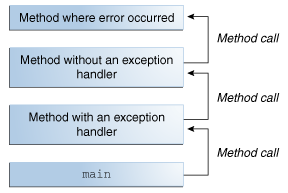
\includegraphics[width=0.8\linewidth]{figs/exceptions-callstack.png}

  	\column{.50\textwidth}
		\textit{Call stack}: Sequence of invoked methods
	\end{columns}
\end{frame}

\begin{frame}{Exceptions}{Exception definition (III)}
    \begin{columns}
 	   \column{.60\textwidth}
		\centering Exception handling
		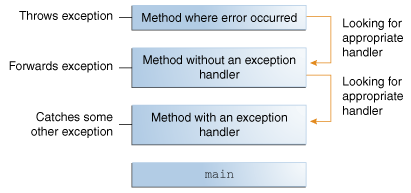
\includegraphics[width=0.8\linewidth]{figs/exceptions-errorOccurs.png}

  	\column{.60\textwidth}
		When an error happens ...
		\begin{enumerate}
		\item Code execution is stopped
		\item An exception is thrown
		\item The interpreter goes back in the call stack
		\item When the interpreter finds an exception handler, it is executed
		\end{enumerate}
		The exception handler catches the exception, the program finishes otherwise
	\end{columns}
\end{frame}

\begin{frame}{Exceptions}{Exception definition (IV)}
	\lstinputlisting{code/stack.txt}
\end{frame}

\section{Handling exceptions}
\begin{frame}{Exceptions}{Handling exceptions (I)}
	Handling an exception requires a try-except statement
	\begin{itemize}
		\item \texttt{try}: Encloses the vulnerable code
		\item \texttt{catch}: Code that handles the exception
	\end{itemize}

    \begin{columns}
 	   \column{.60\textwidth}
	\begin{block}{try-catch statement}
	\vspace{-0.2cm}
		\lstinputlisting{code/try.py}
	\vspace{-0.2cm}
	\end{block}
	\end{columns}
\end{frame}

\begin{frame}{Exceptions}{Handling exceptions (II)}
    \begin{columns}
 	   \column{.90\textwidth}
	\begin{block}{try-catch example}
	\vspace{-0.2cm}
		\lstinputlisting[numbers=left]{code/try-example.py}
	\vspace{-0.2cm}
	\end{block}
	\end{columns}
	\bigskip
	The exception type contains the error
\end{frame}

\begin{frame}{Exceptions}{Handling exceptions (III)}
	\vspace{-0.2cm}
    \begin{columns}
 	   \column{.90\textwidth}
	\begin{block}{try-catch example}
	\vspace{-0.2cm}
		\lstinputlisting[numbers=left]{code/try-example2.py}
	\vspace{-0.2cm}
	\end{block}
	\end{columns}
	\bigskip
	New Python element
		\begin{itemize}
		\item Raise
		\end{itemize}
\end{frame}

\section{Exceptions with arguments}
\begin{frame}{Exceptions}{Exceptions with arguments}
	\vspace{-0.2cm}
	\textit{Exception arguments}: When we need more info


	\vspace{-0.2cm}
    \begin{columns}
 	   \column{.70\textwidth}
	\begin{block}{}
	\vspace{-0.2cm}
		\lstinputlisting[numbers=left]{code/try-arg.py}
	\vspace{-0.2cm}
	\end{block}

	\vspace{-0.3cm}

	\begin{block}{}
	\vspace{-0.2cm}
		\lstinputlisting[numbers=left]{code/try-arg-res.py}
	\vspace{-0.2cm}
	\end{block}

	\end{columns}
\end{frame}

\section{Clean-up actions}
\begin{frame}{Exceptions}{Clean-up actions}
	\vspace{-0.2cm}
	Sometimes we need to execute code under all circumstances
	\begin{itemize}
		\item Typically clean-up actions: Close files, database connections, sockets, etc
		\item The \textbf{finally} clause solves this problem
	\end{itemize}

	\vspace{-0.2cm}
    \begin{columns}
 	   \column{.60\textwidth}
	\begin{block}{Example}
	\vspace{-0.2cm}
		\lstinputlisting[numbers=left]{code/try-finally.py}
	\vspace{-0.2cm}
	\end{block}

	\end{columns}
\end{frame}



\end{document}
